\documentclass[]{article}
\usepackage{graphicx}
\usepackage{hyperref}
\usepackage{float}

%opening
\title{Assignment 2 CDA}
\author{Tim van Rossum, 4246306\\
	Michiel Doesburg, 4343875}

\begin{document}

\maketitle
\section{Familiarization with the data}
The dataset contains a total of 44 signals, with some being static values, other being sinusoid signals, and others being partially discrete (as in, they can rise or drop at certain points). L-signals tend to be more sinusoidal, F-signals tend to be "partially discrete", and S-signals are all binary signals. Figure 1 shows some of the signals, while figure 2 also shows the ARMA predictions for these signals. As can be seen from figure 1, some signals are strongly correlated, especially F\_PU1 and F\_PU2, which have a correlation of almost -1. Figure 2 also shows that ARMA performs better predicting the more sinusoidal signals, as the prediction for L\_T1 is significantly better than the prediction for the other two signals.

% All the signals together seem to have little correlation. Some combinations of signals are reasonably correlated: e.g. L\_T3 and P\_J302 have a 0.42 correlation coefficient. Moreover, the signal P\_J302 in figure~\ref{correlation} looks cyclic. A cyclic signal like this is much easier to predict than a `random' signal, since there is a rough base model that it adheres to. This signal's values are within a clear band at about 2-6 on the Y-axis. In such a case it is very easy to come up with a basic anomaly detection technique: if the signal moves outside this band this would be a clear sign of an anomaly. Plotting the mean error we saw for the ARMA prediction on signal L\_T1, we saw that there were only 2 cases were the error was greater than three times the standard deviation. 

\begin{figure}[H]
\begin{minipage}{.5\textwidth}
  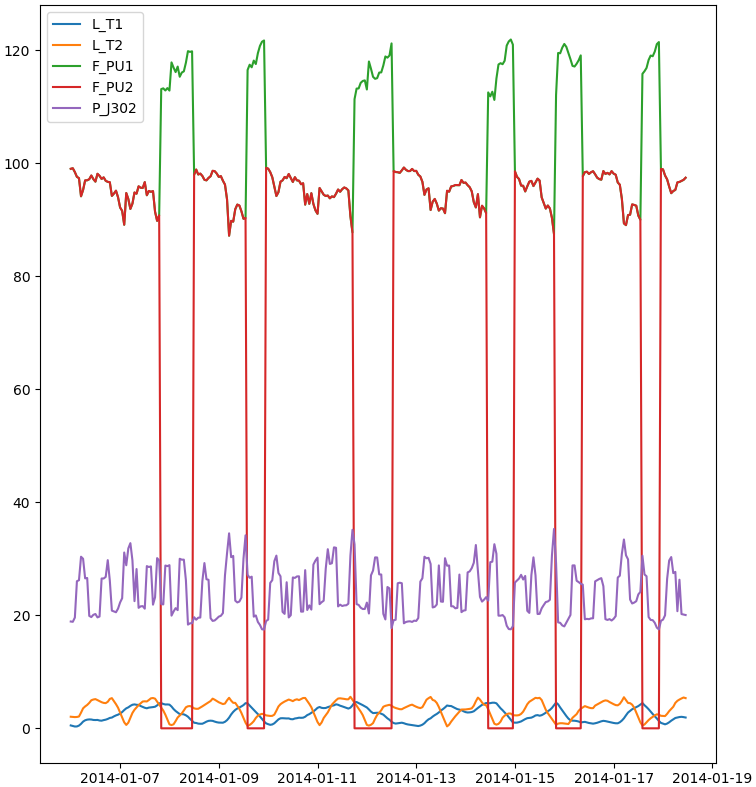
\includegraphics[width=0.8\linewidth, height=4cm]{./visuallizations/signals.png}
  \caption{Visualization of some signals. The red and greens signals are partially discrete.}
  \label{signals}
\end{minipage} %
\begin{minipage}{.5\textwidth}
  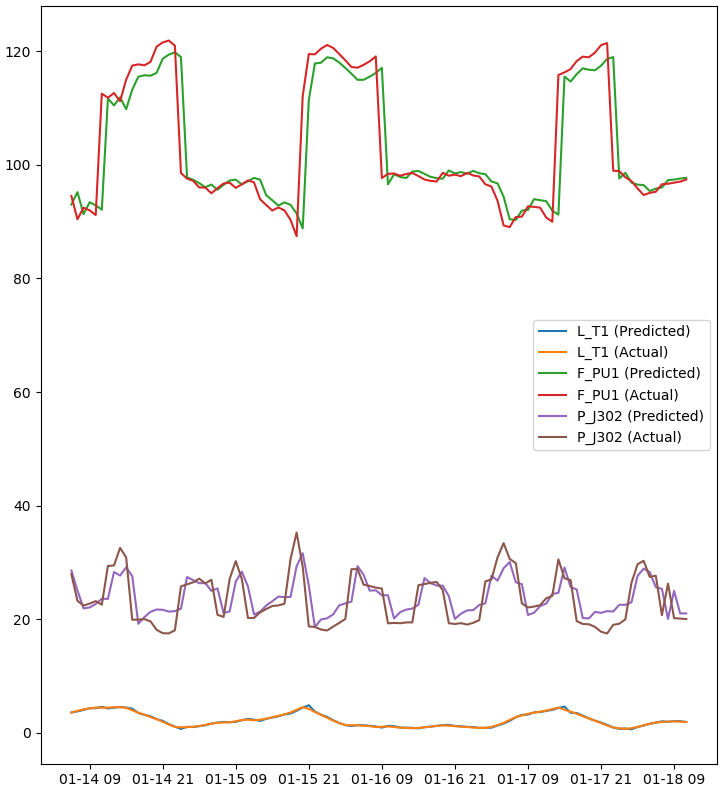
\includegraphics[width=0.8\linewidth, height=4cm]{./visuallizations/predictions.png}
   \caption{ARMA predictions on some signals. The predictions work better on signals.with less variance}
  \label{predictions}
\end{minipage}
%\begin{minipage}{.5\textwidth}
  %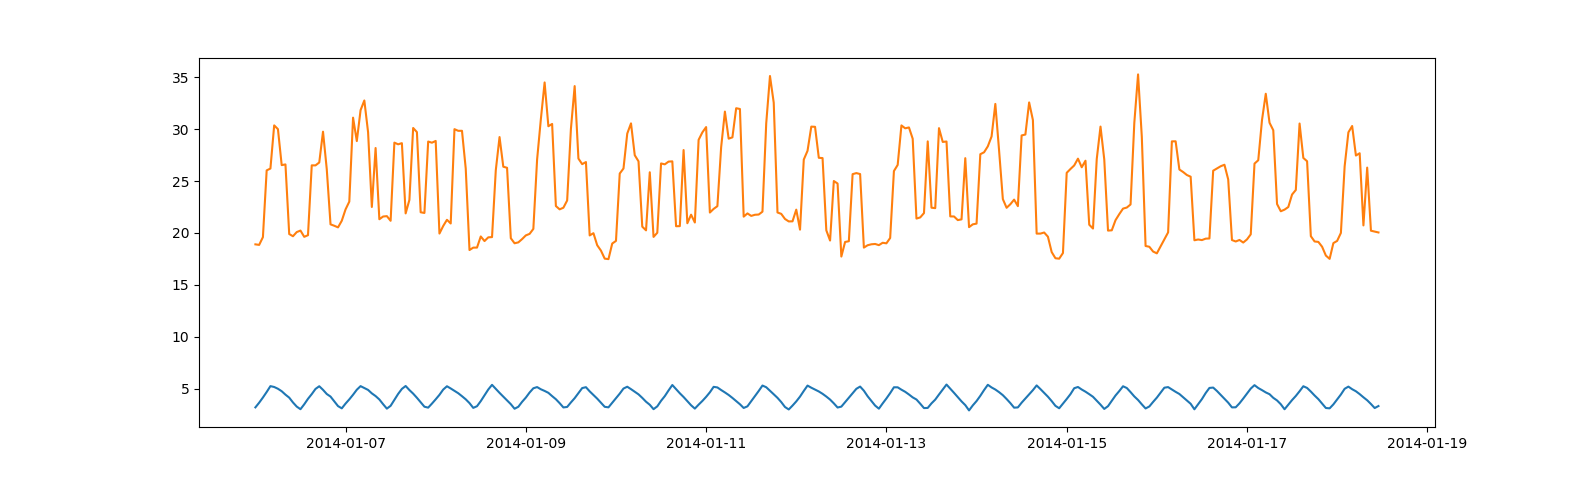
\includegraphics[width=2\linewidth, height=3.5cm]{./visuallizations/correlated_signals.png}.
  %\label{correlation}
  %\caption{Signals L\_T3 and P\_J302. The peaks are roughly aligned.}
%\end{minipage}%
\end{figure}
\clearpage
\section{ARMA}
The script \texttt{ARMA.py} learns a ARMA model for any particular sensor. The parameters for the model are determined by testing out different $p$'s and $q$'s and then looking at the AIC value of the fitted model. A lower AIC means a better fit. Fitting the models takes quite some time, and as such the search space for parameters is limited. For $p$, only values in the range of $[0, 8]$ are tested, and for $q$, only values in the range of $[0, 2]$ are tested. Both these ranges are inclusive. We thought these ranges would still allow for a reasonable search space while limiting the time taken to search for the ideal parameters.

After the predictions are done, the predicted values are compared to the actual values. The difference between the two is used, and then the mean of the absolute values is computed, along with the standard deviation of the absolute values. An attack is detected if a predicted value differs from the actual value by more than the absolute mean plus three times the standard deviation. The sensors that have cyclic time series can be modelled effectively by ARMA, and the anomalies that can be detected are contextual anomalies.
\section{Discrete models}
For this task, we used the SAX method as shown in class. The script \texttt{SAX.py} is a script that can discretize a time series using SAX. The script was provided by Qin Lin, and we altered a few things to make it work with Python 3. Discretization of the signal in this way creates a representative string of characters of the signal, which allows us to perform sequential data mining methods on it. This is in contrast to PAA, which only discretizes the signal, which does not allow us to perform these data mining methods. Discretization by use of SAX makes sense as the signal values are now grouped by how much they differ from the mean of the signal. The window size determines how many mean values the signal will be converted to, and the amount of original data points used per mean. Using a very large window size will obviously result in a very rough approximation and much data loss, using a very small window size will simply approach the original data and be pointless. After some trial-and-error, we found a window size of 3 to work well. The alphabet size determines the range of possible discrete values the means will be mapped to. 

The script \texttt{applying\_SAX.py} does not only apply SAX on the signals, but also applies the N-grams data mining method to find anomalies. An N-gram is anomalous (and possibly an indicator of an attack) if the score is lower than either the mean score minus three times the standard deviation, or 0.3, whichever is higher. The 0.3 was chosen to prevent the score boundary from becoming negative. It is rather rare to have that happen on this data though, as having large word sizes allows us to have a mean score of around 0.98 for most signals with a standard deviation of about 0.2. The sensors that do not have cyclic time series can be modelled effectively by SAX, and the anomalies that can be detected are collective anomalies.
\clearpage
\section{PCA}
For this task, we first transformed the dataset using PCA. Before applying PCA, we set the mean of all the signals to 0. We do not divide the signals by their standard deviation as some signals have a standard deviation of 0 and working around this by dividing the time series only when the standard deviation is non-zero causes the isolation forest to not detect anything at all any more. The procedure can be found in the script \texttt{PCA.py}. We used the PCA implementation in Scikit-learn because we use Python as our platform. After the dataset was transformed, we could perform outlier detection. Scikit-learn also has several methods for that: one-class SVM, isolation forest, elliptic envelope, and local outlier factor. We decided to use the methods shown in class, which were the one-class SVM and the isolation forest. The isolation forest model finds significantly less anomalies than the one-class SVM model, possibly making the isolation forest model better in this case.

The workflow is as follows: the models are first fitted on the transformed dataset that contains no attacks whatsoever (which is the first of the BATADAL training datasets). Then, predictions are made for the transformed test dataset. If an index is predicted to be an outlier, then the timestamp is stored in a list. TODO plot of PCA residuals. Using PCA, we can detect point anomalies.
\clearpage
\section{Comparison} 

\end{document}
